\subsection{Methods}
For the third week, I worked on alpha-beta pruning for the minimax algorithm. Once this was completed, I updated the board hash to store a \texttt{hash} variable, which updates with each move, rather than rehashing completely each time. When using the alpha-beta algorithm, only some states could be cached (i.e., those without pruned descendants), in order to avoid copying faulty scores across the tree to a state where pruning should not be applied.

I also added an evaluation function, by which moves would be ordered. This works separately from the result function (leaf nodes), but does begin by checking if the game is in a terminal state and returning \(-\infty\), \(0\), or \(\infty\) when appropriate. Otherwise, all game lines are considered, and if the opponent has the opportunity to win in the next move, \(-\infty\) is returned. If the current player has a fork (two opportunities to win, so the opponent has no chance), \(\infty\) is returned. Otherwise, for each line that the player or opponent has control over, the number of squares taken in that line is added/subtracted (respectively) from the score. This score is then returned as the evaluation.

As shown by the following results, more improvements may need to be made to the evaluation function. This can be achieved through further testing and experimentation. 

\subsection{Results}

The following graph shows the result of applying pruning (without cache). This is most effective on the first move, where the pruned method visits only about 5\% as many states as the original minimax algorithm.

\begin{center}
    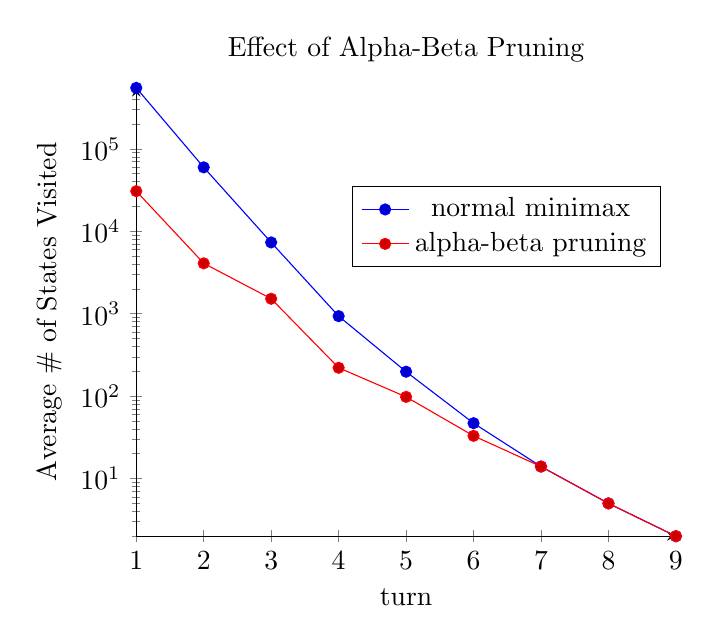
\begin{tikzpicture}
        \begin{axis}[
            legend style={at={(.4,.6)},anchor=south west},
            axis lines = left,
            xlabel = turn,
            xtick = {0, 1, 2, 3, 4, 5, 6, 7, 8, 9},
            ymode = log,
            ylabel = Average \# of States Visited,
            title = Effect of Alpha-Beta Pruning
        ]
        \addplot+[
            mark=*,
        ] plot coordinates{
            (1,549946)
            (2,59705)
            (3,7332)
            (4,935)
            (5,198)
            (6,47)
            (7,14)
            (8,5)
            (9,2)
        };
        \addlegendentry{normal minimax}
        \addplot+[
            mark=*,
        ] plot coordinates{
            (1,30710)
            (2,4090)
            (3,1520)
            (4,221)
            (5,98)
            (6,33)
            (7,14)
            (8,5)
            (9,2)
        };
        \addlegendentry{alpha-beta pruning}
        
        \end{axis}
    \end{tikzpicture}
\end{center}

Caching did eliminate a few thousand states, but did not make a large difference due to the fact that not many states were cached. Note that there are still some uncached states visited after move 2, due to the fact that not all states were cached (those with pruned descendants were not).

\begin{center}
    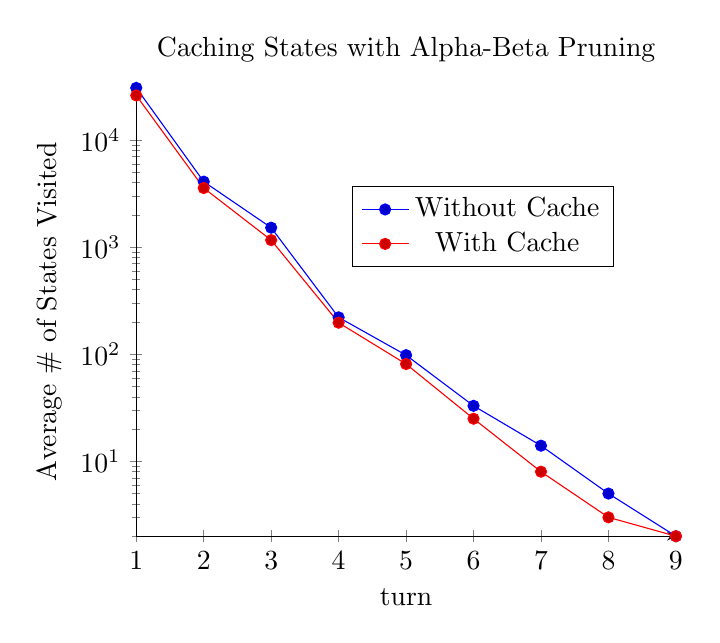
\begin{tikzpicture}
        \begin{axis}[
            legend style={at={(.4,.6)},anchor=south west},
            axis lines = left,
            xlabel = turn,
            xtick = {0, 1, 2, 3, 4, 5, 6, 7, 8, 9},
            ymode = log,
            ylabel = Average \# of States Visited,
            title = Caching States with Alpha-Beta Pruning
        ]
        \addplot+[
            mark=*,
        ] plot coordinates{
            (1,30710)
            (2,4090)
            (3,1520)
            (4,221)
            (5,98)
            (6,33)
            (7,14)
            (8,5)
            (9,2)
        };
        \addlegendentry{Without Cache}
        \addplot+[
            mark=*,
        ] plot coordinates{
            (1,26089)
            (2,3565)
            (3,1163)
            (4,197)
            (5,81)
            (6,25)
            (7,8)
            (8,3)
            (9,2)
        };
        \addlegendentry{With Cache}
        
        \end{axis}
    \end{tikzpicture}
\end{center}

The next graph highlights that the new hashing method (storing the hash rather than rehashing) has a consistent runtime improvment.

\begin{center}
    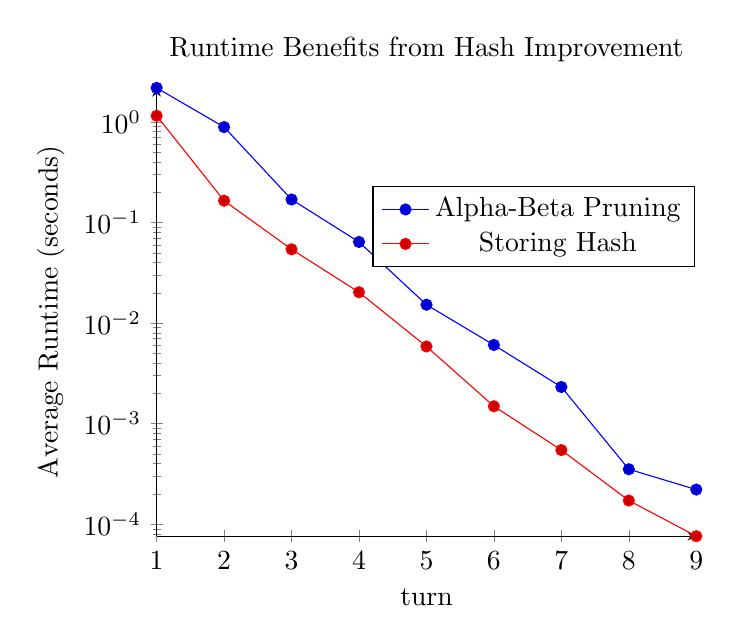
\begin{tikzpicture}
        \begin{axis}[
            legend style={at={(.4,.6)},anchor=south west},
            axis lines = left,
            xlabel = turn,
            xtick = {0, 1, 2, 3, 4, 5, 6, 7, 8, 9},
            ymode = log,
            ylabel = Average Runtime (seconds),
            title = Runtime Benefits from Hash Improvement
        ]
        \addplot+[
            mark=*,
        ] plot coordinates{
            (1,2.183425)
            (2,0.889763)
            (3,0.169497)
            (4,0.064108)
            (5,0.015237)
            (6,0.006057)
            (7,0.002315)
            (8,0.000352)
            (9,0.000221)
        };
        \addlegendentry{Alpha-Beta Pruning}
        \addplot+[
            mark=*,
        ] plot coordinates{
            (1,1.151719)
            (2,0.164936)
            (3,0.054198)
            (4,0.020260)
            (5,0.005853)
            (6,0.001489)
            (7,0.000546)
            (8,0.000172)
            (9,0.000076)
        };
        \addlegendentry{Storing Hash}
        
        \end{axis}
    \end{tikzpicture}
\end{center}

The following graph shows a comparision of states visited from a normal alpha-beta search, and two searches where moves are ordered by the current evaluation, in both a normal/positive and a reverse/negative fashion. All of these were done without a cache. There is a fairly consistent improvement caused by move ordering. Although the scale under-exaggerates it, move ordering visits just 25\% as many states as the default order.

\begin{center}
    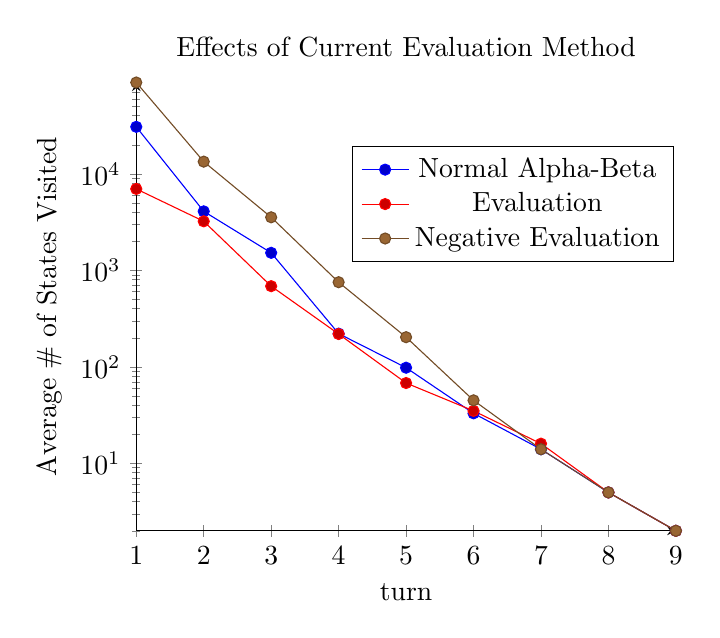
\begin{tikzpicture}
        \begin{axis}[
            legend style={at={(.4,.6)},anchor=south west},
            axis lines = left,
            xlabel = turn,
            xtick = {0, 1, 2, 3, 4, 5, 6, 7, 8, 9},
            ymode = log,
            ylabel = Average \# of States Visited,
            title = Effects of Current Evaluation Method
        ]
        \addplot+[
            mark=*,
        ] plot coordinates{
            (1,30710)
            (2,4090)
            (3,1520)
            (4,221)
            (5,98)
            (6,33)
            (7,14)
            (8,5)
            (9,2)
        };
        \addlegendentry{Normal Alpha-Beta}
        \addplot+[
            mark=*,
        ] plot coordinates{
            (1,6982)
            (2,3224)
            (3,686)
            (4,219)
            (5,68)
            (6,35)
            (7,16)
            (8,5)
            (9,2)
        };
        \addlegendentry{Evaluation}
        \addplot+[
            mark=*,
        ] plot coordinates{
            (1,88500)
            (2,13391)
            (3,3548)
            (4,754)
            (5,203)
            (6,45)
            (7,14)
            (8,5)
            (9,2)
        };
        \addlegendentry{Negative Evaluation}
        
        \end{axis}
    \end{tikzpicture}
\end{center}

This evaluation results in the following board state, with the first move occuring in the middle cell (with the highest heuristic):

\[
\begin{array}{c|c|c}
    \textbf{o} & \textbf{x} & \textbf{x}\\
    \hline
    \textbf{x} & \textbf{x} & \textbf{o}\\
    \hline
    \textbf{o} & \textbf{o} & \textbf{x}
\end{array}    
\]

The reverse evaluation ends in this state, with the first move being in the middle of the top row (tied for lowest heuristic value):

\[
\begin{array}{c|c|c}
    \textbf{o} & \textbf{x} & \textbf{o}\\
    \hline
    \textbf{x} & \textbf{o} & \textbf{x}\\
    \hline
    \textbf{x} & \textbf{o} & \textbf{x}
\end{array}    
\]